\textbf{Pour cette première partie, aucune justification n'est demandée et une seule réponse est possible par question. Pour chaque question, reportez son numéro sur votre copie et indiquez votre réponse.}

\subsubsection*{Question 1}
L'opération qui permet de calculer 25\% de 480 est :

\textbf{a.} $\dfrac{480}{25 \times 100}$ \hfill \textbf{b.} $25 \times 480 \times 0,1$ \hfill 
\textbf{c.} $\dfrac{480 \times 100}{25}$ \hfill \textbf{d.} $\dfrac{1}{4} \times 480$

\subsubsection*{Question 2}
Voici trois nombres.

$A = \dfrac{1}{5}$ \hfill $B = \dfrac{19}{100}$ \hfill $C = 0,21$

Le classement par ordre croissant de ces trois nombres est :

\textbf{a.} $A < B < C$ \hfill \textbf{b.} $A < C < B$ \hfill 
\textbf{c.} $B < A < C$ \hfill \textbf{d.} $C < B < A$

\subsubsection*{Question 3}
Voici quatre nombres.

$A = \left(\dfrac{1}{5}\right)^2$ \hfill $B = \left(\dfrac{1}{2}\right)^5$ \hfill $C = 0,05$ \hfill $D = \left(\dfrac{1}{3}\right)^3$

Le plus grand de ces quatre nombres est :

\textbf{a.} $A$ \hfill \textbf{b.} $B$ \hfill \textbf{c.} $C$ \hfill \textbf{d.} $D$

\subsubsection*{Question 4}
Un article augmente de 10\% puis il augmente encore de 10\%. Après ces deux augmentations il a augmenté de :

\textbf{a.} $(10\%)^2$ \hfill \textbf{b.} $19\%$ \hfill \textbf{c.} $20\%$ \hfill \textbf{d.} $21\%$

\subsubsection*{Question 5}
Le tiers d'un quart correspond à la fraction :

\textbf{a.} $\dfrac{1}{7}$ \hfill \textbf{b.} $\dfrac{3}{4}$ \hfill \textbf{c.} $\dfrac{1}{3} \times 4$ \hfill \textbf{d.} $\dfrac{1}{12}$

\subsubsection*{Question 6}
On considère $A = 10 + 0,1 + \dfrac{1}{1000}$. On a :

\textbf{a.} $A = \dfrac{20^{- 1}}{1000}$ \hfill \textbf{b.} $A = \dfrac{1}{1000}$ \hfill 
\textbf{c.} $A = 10,101$ \hfill \textbf{d.} $A = 10,110$

\subsubsection*{Question 7}
On considère $A = 10^{10} + 10^{-10}$. $A$ est environ égal à :

\textbf{a.} $10^0$ \hfill \textbf{b.} $0$ \hfill \textbf{c.} $10^{10}$ \hfill \textbf{d.} $100^0$

\subsubsection*{Question 8}
Une durée de 100 minutes correspond à :

\textbf{a.} 1 heure \hfill \textbf{b.} 1,40 heure \hfill 
\textbf{c.} $\dfrac{5}{3}$ heure \hfill \textbf{d.} 2 heures

\bigskip

\begin{minipage}[t]{0.7\textwidth}
\subsubsection*{Question 9}
On considère une droite $D$ représentée ci-contre.

La seule équation pouvant correspondre à l'équation réduite de la droite $D$ est :

\textbf{a.} $y = x + 3$ \hfill \textbf{b.} $y = x - 3$ \hfill 
\textbf{c.} $y = -x + 3$ \hfill \textbf{d.} $y = -x - 3$
\end{minipage}
\hfill
\begin{minipage}[t]{0.29\textwidth}
\vspace{0pt}
\begin{center}
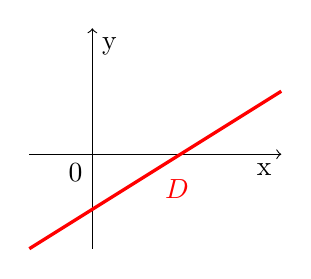
\begin{tikzpicture}[scale=0.8]
\draw[->] (-1,0) -- (3,0) node[below left] {x};
\draw[->] (0,-1.5) -- (0,2) node[below right] {y};
\draw[very thick, color=red] (-1,-1.5) -- (3,1);
\node[below left] at (0,0) {0};
\node[below right, color=red] at (1,-0.25) {$D$};
\end{tikzpicture}
\end{center}
\end{minipage}

\subsubsection*{Question 10}
On considère la fonction $f$ définie pour tout réel $x$ par $f(x) = 7 - \dfrac{1}{2}(x - 3)^2$.

L'image de 3 par la fonction $f$ est égale à :

\textbf{a.} $7 - \dfrac{1}{2}$ \hfill \textbf{b.} $7 - \dfrac{1}{2}(9 + 9)$ \hfill 
\textbf{c.} $7$ \hfill \textbf{d.} $0$

\subsubsection*{Question 11}
Quand on développe $(x - 3)^2$ on obtient :

\textbf{a.} $x^2 + 9$ \hfill \textbf{b.} $x^2 - 9$ \hfill 
\textbf{c.} $x^2 + 6x - 9$ \hfill \textbf{d.} $x^2 - 6x + 9$

\subsubsection*{Question 12}
Voici deux séries de valeurs.

Série A : 1 ; 2 ; 3 \hfill Série B : 0,5 ; 2 ; 100

Une seule de ces affirmations est exacte :

\textbf{a.} Les deux séries ont la même moyenne et la même médiane. \\
\textbf{b.} Les deux séries ont la même moyenne mais pas la même médiane. \\
\textbf{c.} Les deux séries ont la même médiane mais pas la même moyenne. \\
\textbf{d.} Les deux séries n'ont ni la même moyenne ni la même médiane.
